\documentclass{article}
\usepackage{graphicx}
\usepackage{amsmath}
\usepackage{hyperref}
\usepackage{siunitx}
\usepackage[super]{nth}
\usepackage{pgfplots}
\usepackage{filecontents}
\usepackage{listings}
%\graphicspath{{../images/} }

%-------------------------------------------------------------------------------
%	TITLE SECTION
%-------------------------------------------------------------------------------

\newcommand{\horrule}[1]{\rule{\linewidth}{#1}} % Create horizontal rule command with 1 argument of height
\title{
\normalfont \normalsize
\textsc{Sapienza University of Rome} \\ [25pt]
\horrule{0.5pt} \\[0.4cm] % Thin top horizontal rule
\LARGE Modern Portfolio Theory \\
\large Visual Analytics \\
\horrule{2pt} \\[0.5cm] % Thick bottom horizontal rule
}

\author{Ibis Prevedello}
\date{\normalsize\today}

\begin{document}
\maketitle

%-------------------------------------------------------------------------------
%	REPORT SECTION
%-------------------------------------------------------------------------------

\section{Abstract}
Choosing the correct investment portfolio to have is a really difficult task, this is the first and most difficult thing to define, because once that it is set, the investor's task is basically to follow it.
There are different ways and analysis to make in order to define a portfolio allocation, one of them is known as Modern Portfolio Theory (MPT), and this is the one that is implemented in this software as well as here described.

\section{Introduction}
Modern Portfolio Theory (MPT) is a theory on how investors can construct portfolios to optimize or maximize expected return based on a given level of market risk, emphasizing that risk is an inherent part of higher reward. According to the theory, it is possible to construct an "efficient frontier" of optimal portfolios offering the maximum possible expected return for a given level of risk. This theory was pioneered by Harry Markowitz in his paper "Portfolio Selection" \cite{doi:10.1111/j.1540-6261.1952.tb01525.x}, published in 1952 by the Journal of Finance. He was later awarded a Nobel prize for developing the MPT.

MPT shows that an investor can construct a portfolio of multiple assets that will maximize returns for a given level of risk. Likewise, given a desired level of expected return, an investor can construct a portfolio with the lowest possible risk. Based on statistical measures such as variance and correlation, an individual investment's return is less important than how the investment behaves in the context of the entire portfolio.

The risk and return of every possible combination of assets can be plotted in a risk return graph, with the risk on the X-axis and the return Y-axis. From this point it can be analyzed and decide on the correct allocation in order to maximize expected return given a maximum risk one is willing to take or to minimize the risk given the expected return.

\section{Development}

The software developed for this analysis constitutes of four main parts, the first presents the Principal Component Analysis (PCA), the second shows the risk return graph for the assets chosen, the third show the evolution of both assets separately and in the portfolio composition and lastly the portfolio evolution using the Dollar Cost Averaging (DCA) method.

\subsection{Principal Component Analysis (PCA)}

Principal Component Analysis (PCA), is a dimensionality-reduction method that is often used to reduce the dimensionality of large data sets, by transforming a large set of variables into a smaller one that still contains most of the information in the large set.

For this part analysis a dataset of the return of the S&P 500 \cite{sep} was used. The S&P is a stock market index that measures the stock performance of 500 large companies listed on stock exchanges in the United States.

The PCA was used given the correlation matrix of the return of the last 5 years in order to distance the companies based on their return value. The graph presenting the first two components of the PCA is shown in figure \ref{fig:pca} and from this graph it is possible to select two assets for the next analysis.

\begin{figure}
  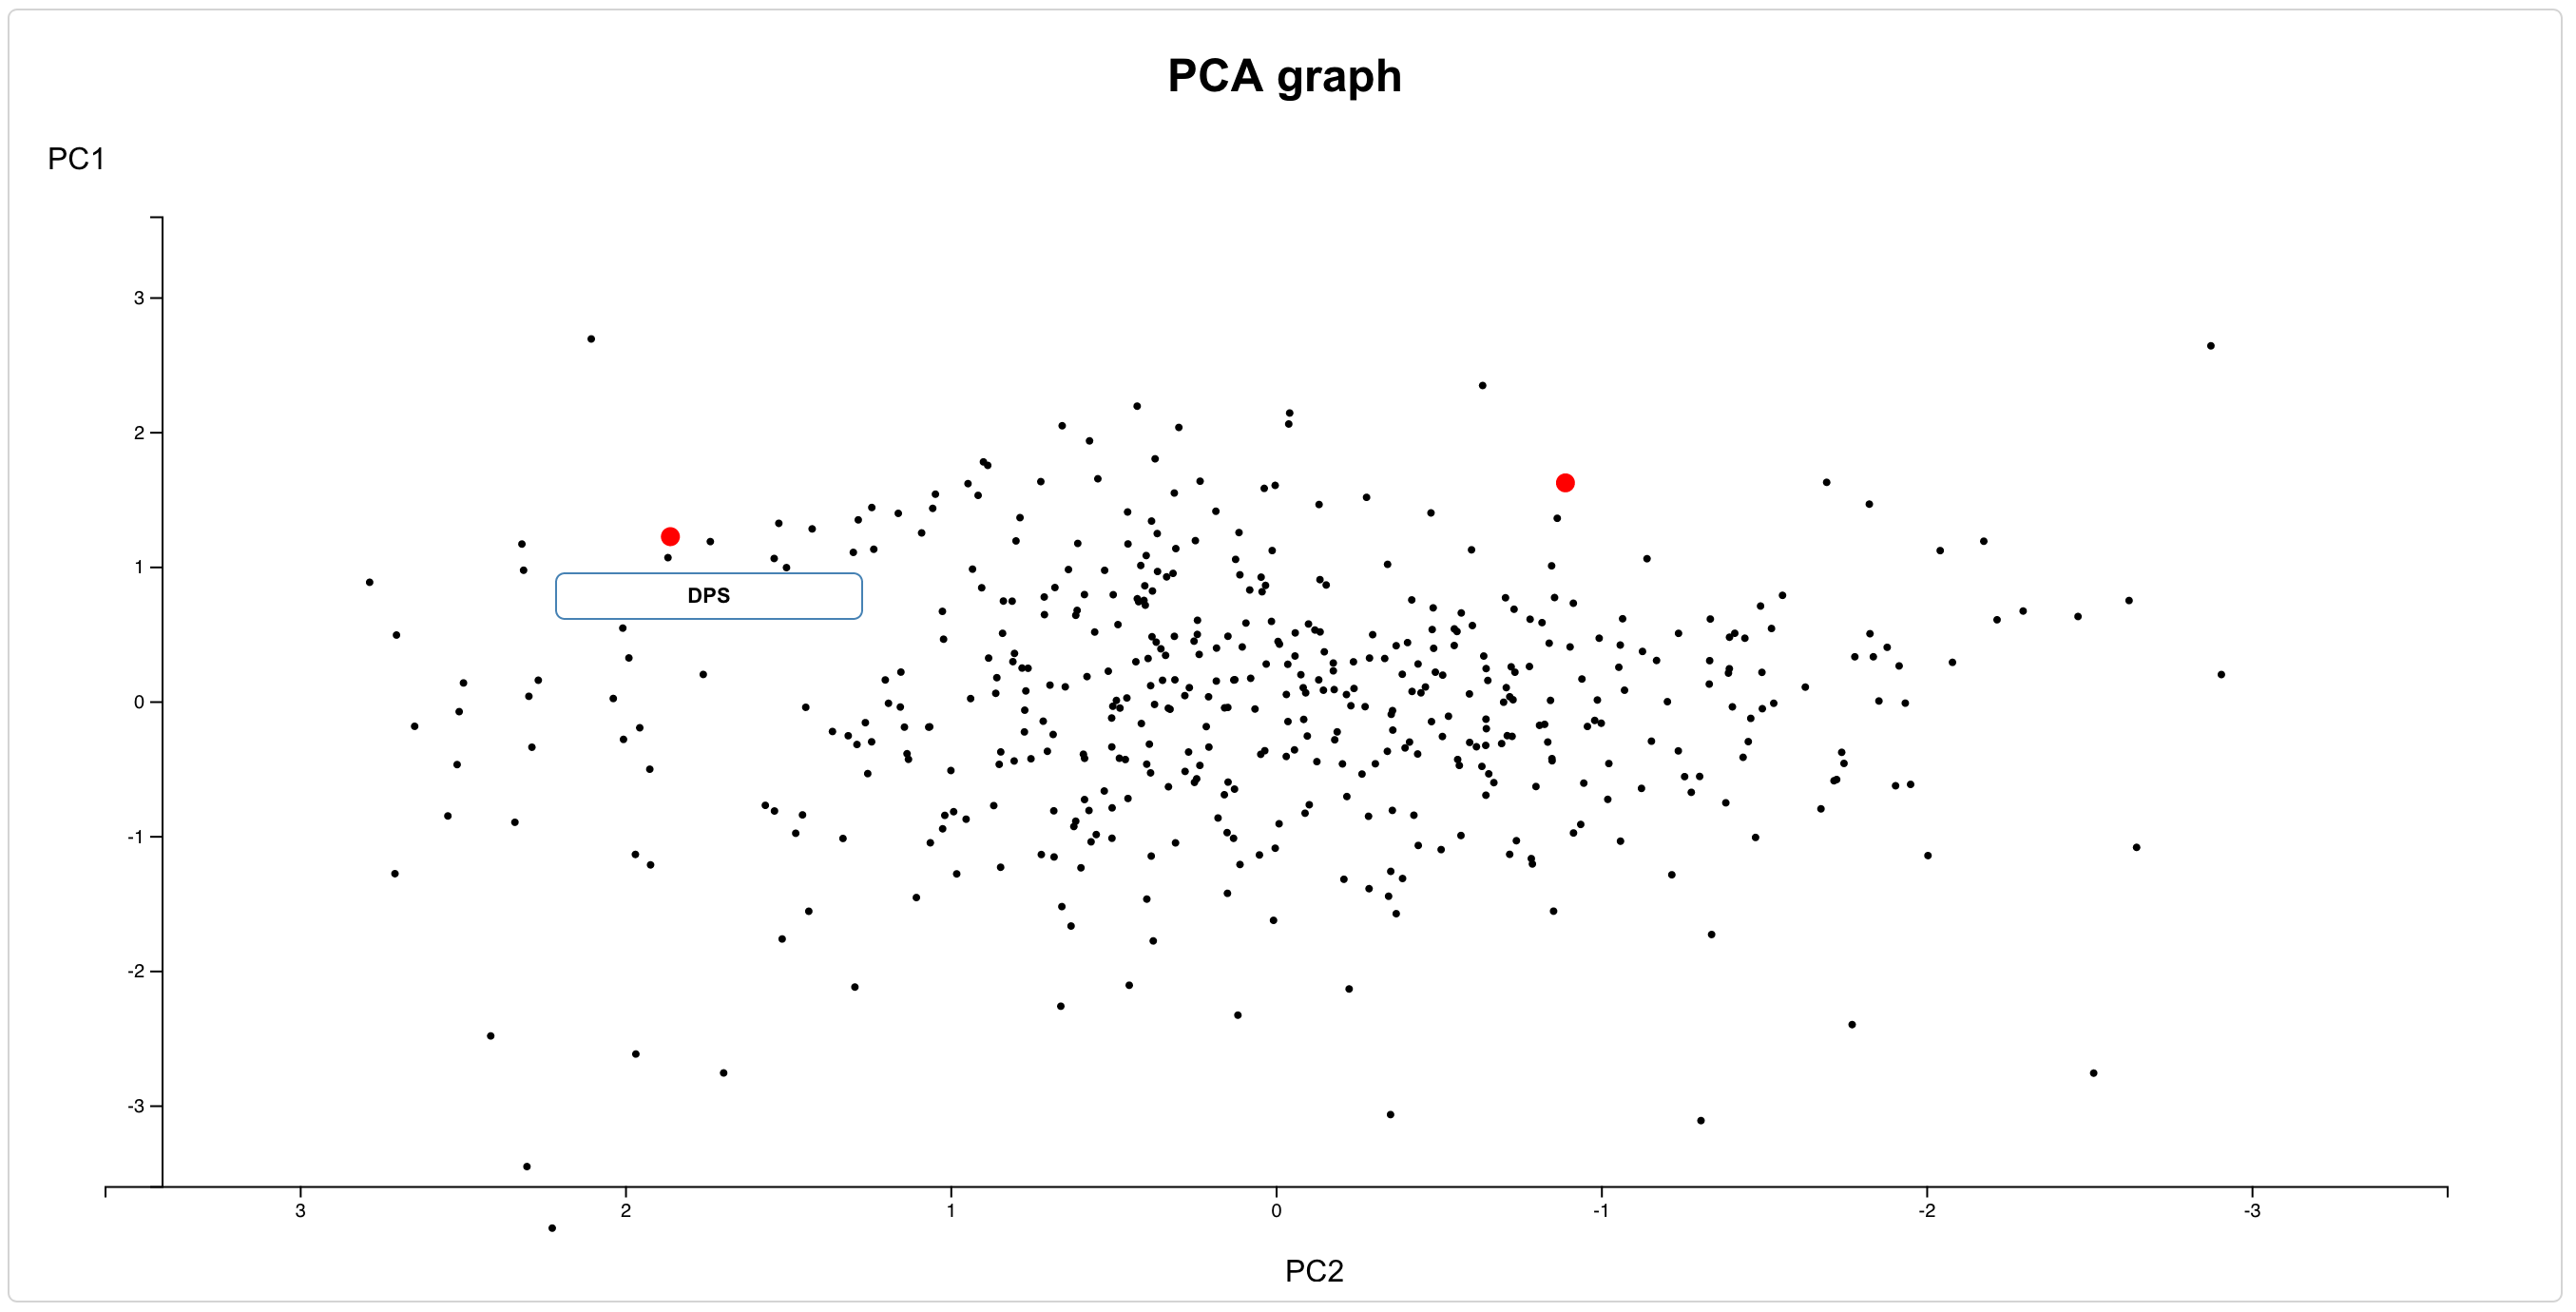
\includegraphics[scale=0.25]{images/pca.png}
  \centering
  \caption{Principal Component Analysis (PCA).}
  \label{fig:pca}
\end{figure}

\subsection{Risk Return}

The second part is the one that implements indeed the risk return graph described by the Modern Portfolio Theory, show in figure \ref{fig:mpt}. Here the user can select two assets from the PCA graph or search for it in the search boxes.

The graph is plotted with 10 dots and a line connecting them, each point varies from 10\% the allocation between the two assets, being the first point 100\% allocated in asset 1 and 0\% allocated to asset 2 and the last point 0\% allocated to asset 1 and 100\% allocated to asset 2.

The line in red represents the Efficient Frontier (EF) which is the maximum return that can be obtained with the minimum possible risk. So, if the investor is more conservative and he needs to choose an allocation given two assets, the best allocation would be the one in the Efficient Frontier.

This and the further graphs are using data requested from Alpha Vantage \cite{alpha_vantage} using an API. The series data used was the Time Series Daily Adjusted, which takes into account split and dividend events.

\begin{figure}
  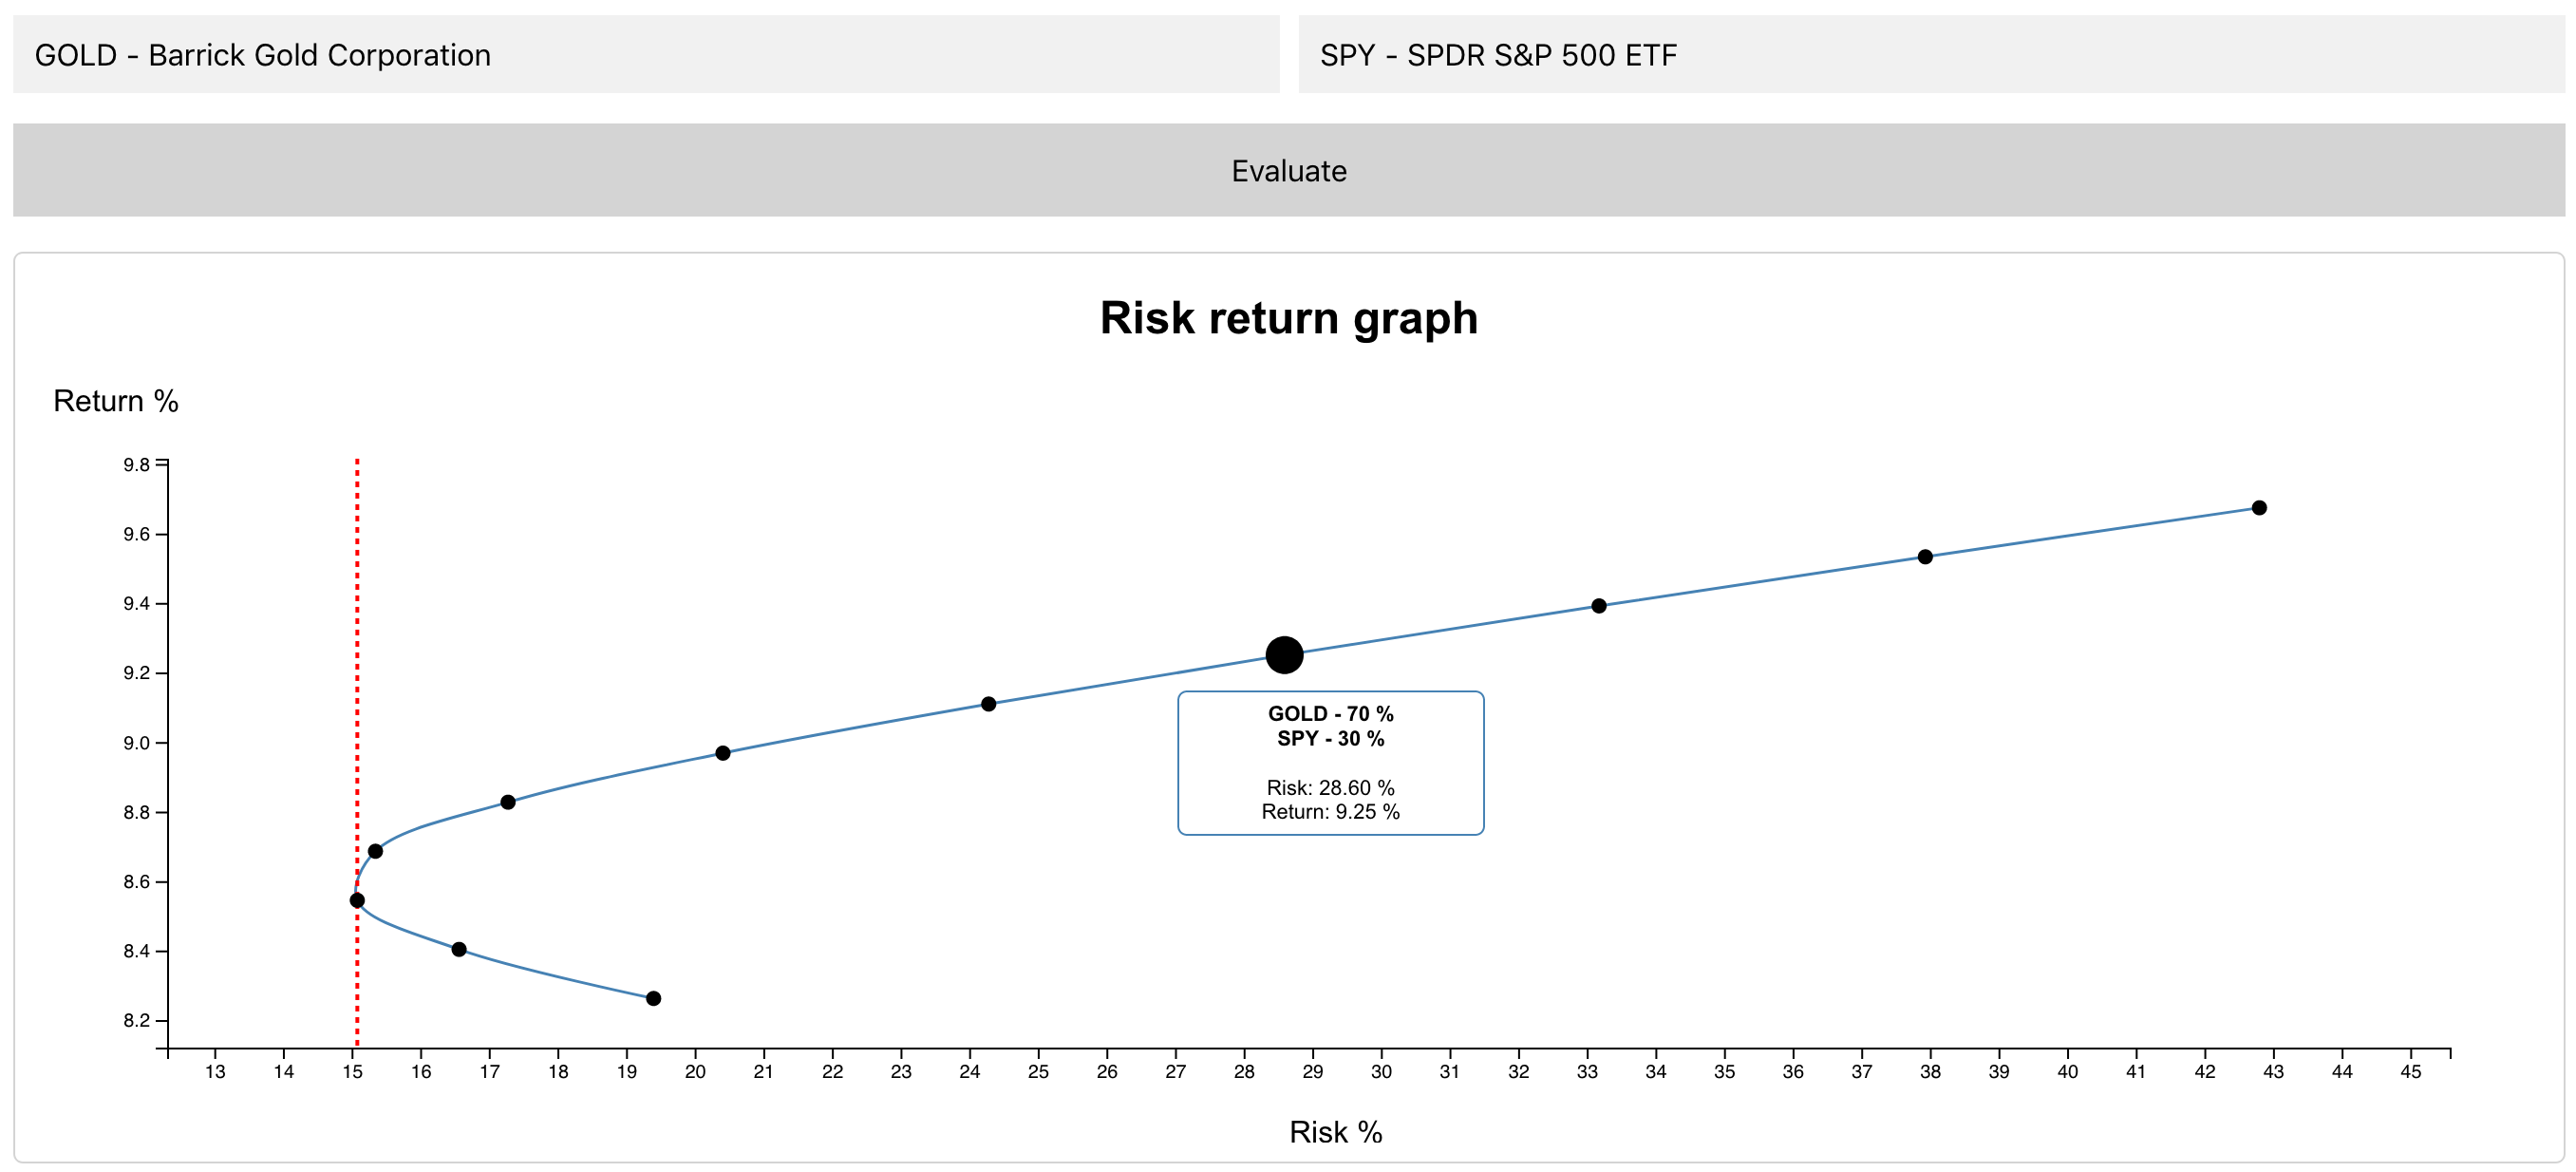
\includegraphics[scale=0.25]{images/mpt.png}
  \centering
  \caption{Risk Return Graph.}
  \label{fig:mpt}
\end{figure}

\subsection{History Graph}

The history graph, shown in figure \ref{fig:history}, simply shows how an investment of 1 dollar in both assets would perform over time, as well as the portfolio chosen from the Risk Return graph. It is possible to change the portfolio allocation simply clicking on the allocation desired and all the other graphs will be updated.

\begin{figure}
  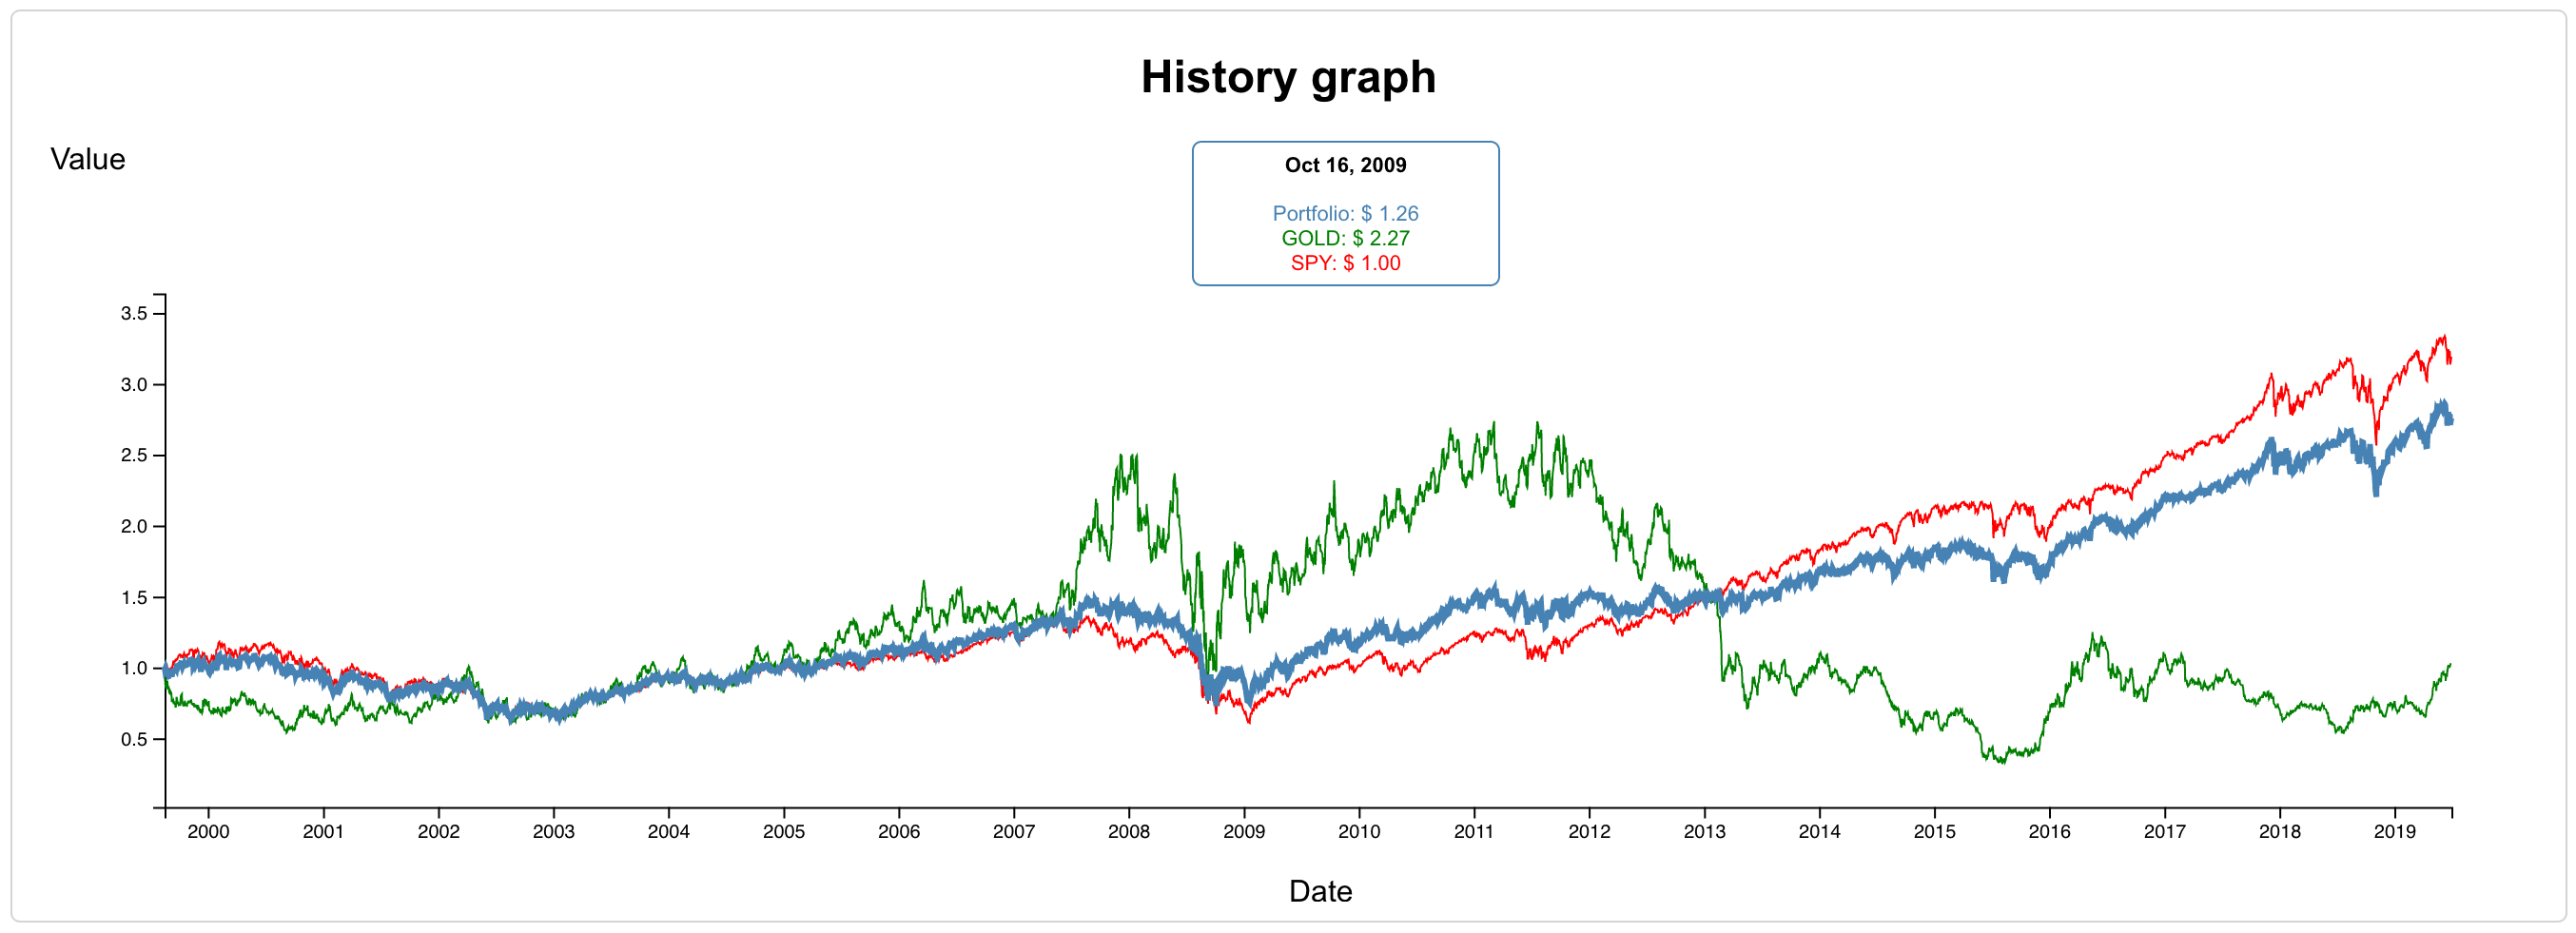
\includegraphics[scale=0.25]{images/history.png}
  \centering
  \caption{History Graph.}
  \label{fig:history}
\end{figure}

\subsection{Dollar Cost Averaging (DCA)}

Dollar Cost Averaging is an investment strategy with the goal of reducing the impact of volatility on large purchases of financial assets, this strategy simulates how a frequent contribution would effect the overall portfolio performance.

This graph, shown in figure \ref{fig:dca}, presents a user interface where it is possible to change the simulation, based on the starting amount, the contribution amount, how often to repeat the contribution and if the user wants to rebalance or not the portfolio.

This periodic contribution works in a way to maintain the percent balance of the portfolio chosen from the Risk Return graph. So, if it was set to maintain the 40\%-60\% allocation rule, the contribution will always be made to the asset that is diverging negatively from this allocation.

For the rebalance, always that the portfolio diverges from 5\% of the allocation defined, it will sell the asset that is above and buy the asset that is below in order to bring back to the desired allocation. This is a very smart strategy, because it forces the investor to always buy when it is low and sell when it is high without having to keep track of the stock market on a daily basis.

This graph also shows some other information as the total invested value, the total portfolio value, the percentage gain or loss and the correlation between the two assets.

The correlation between two assets is a very important aspect to be considered when choosing an asset to add to the portfolio, which varies from -1 to +1, and it is advised to chose assets with negative correlation, which mean that one asset increases in value as the other decreases, and vice versa. Choosing assets with high positive correlation does not make much sense, once it would only cause more transaction costs, not adding any diversification nor risk reduction.

\begin{figure}
  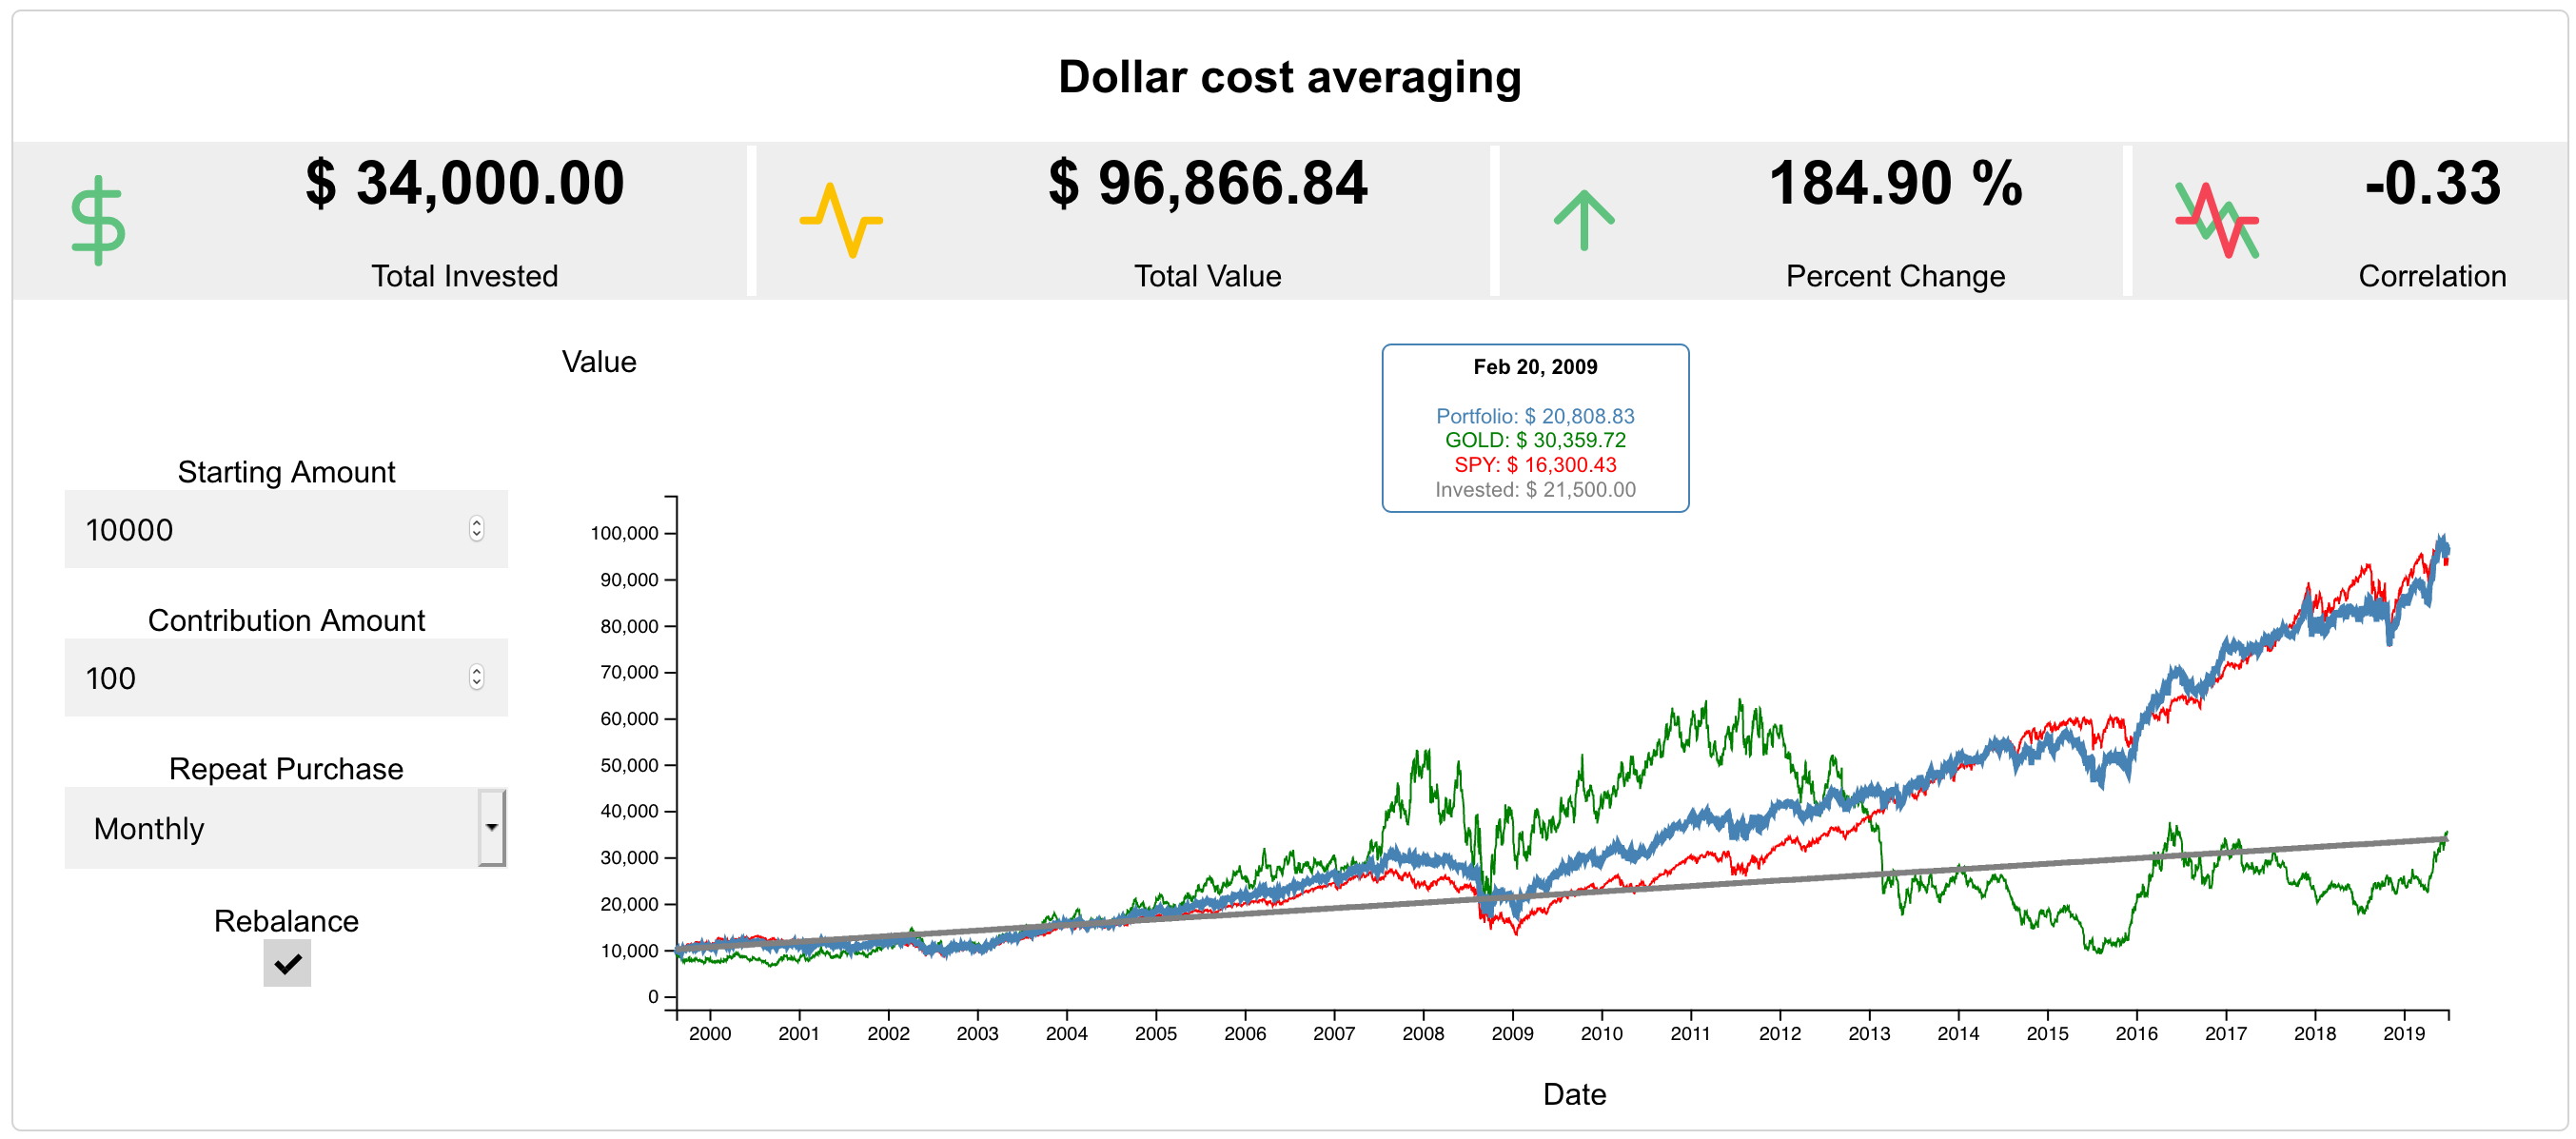
\includegraphics[scale=0.25]{images/dca.png}
  \centering
  \caption{Dollar Cost Averaging.}
  \label{fig:dca}
\end{figure}

\section{Conclusion}

The idea for this project came from the book "All About Asset Allocation" by Richard A. Ferry, this is a book about how to diversify an investment portfolio analyzing the return and the risk of assets based on historical data.

The results here presented show how an easy strategy and tool can change the way people analyze and do investing. In investments there is a maximum that says that past performance is not indicative of future results, but for a long term period when choosing good companies to invest in, it is possible to rely on historical data to have a glance on portfolio performance.

It is also interesting to see how it is possible to outperform assets performance over time using Dollar Cost Averaging. This simple entry strategy shows how important it is the frequency contributions for the long term performance.

\section{Further Improvements}

There are two main improvements that I would like to do for a next version, the first would be the possibility to plot more than two assets for the Risk Return graph and all the other analysis. This would allow to simulate more complex portfolios composed of more assets from different sectors.

The second thing, which is something that limits the implementation of the first one, is to pay for the API in order to have more requests. The free version is limited to only 5 requests per minite and 500 per day, which limits a lot not only the implementation but also the user usability.



%-------------------------------------------------------------------------------
%	BIBLIOGRAPHY SECTION
%-------------------------------------------------------------------------------

\clearpage
\bibliography{bibliography}
\bibliographystyle{ieeetr}

%-------------------------------------------------------------------------------

\end{document}